\documentclass[12pt,letterpaper]{article}
\usepackage{pdfpages}
\usepackage{fancyhdr}
\usepackage[colorlinks=true, urlcolor=blue, linkcolor=blue]{hyperref}
\usepackage{graphicx}
\usepackage[top=1.4in, left=0.5in, right=0.5in, bottom=0.8in]{geometry}
\usepackage[T1]{fontenc}
\usepackage{fontawesome}
\usepackage{helvet}
\pagestyle{fancy}
\renewcommand{\headrulewidth}{0pt}
\renewcommand{\footrulewidth}{0pt}
\setlength{\parindent}{0em}
\setlength{\parskip}{1em}


\fancyfoot[C]{\setlength{\unitlength}{1in}\begin{picture}(5,0)\put(-1.8,-1){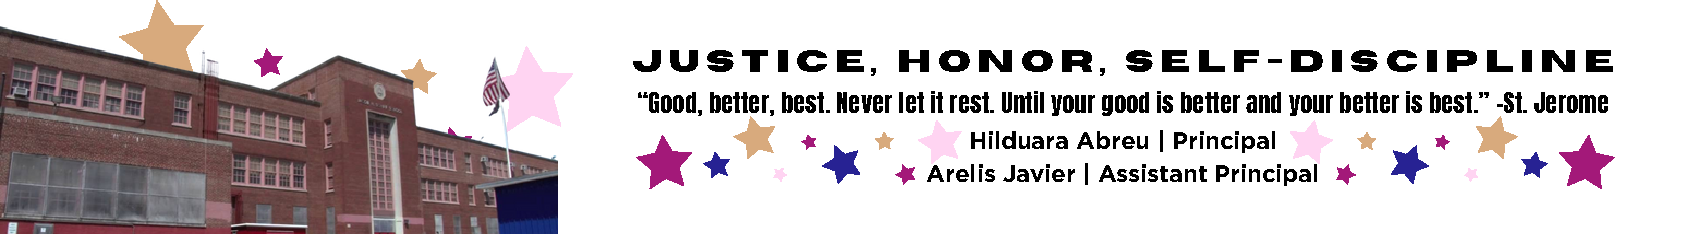
\includegraphics[width=8.8in,height=1.3in]{logo-1}}\end{picture}}
\fancyhead[C]{\setlength{\unitlength}{1in}\begin{picture}(5,0)\put(-1.9,-1){
\includegraphics[width=8.9in,height=1.3in]{logo-2}}\end{picture}}

\pagenumbering{gobble}
\addtolength{\evensidemargin}{-2in}
\addtolength{\topmargin}{-0.5in}
\addtolength{\textwidth}{0in}
%%%%%%%%%%%%%%%%%%%%%%%%%%%%%%%%%%%%%%%%%%%%%%%%%%%%%%%%%%%%%%%%%%

\begin{document}
\vspace*{0.5in}
Date: \href{https://www.ps192.org/}{October, 2023} 

\textbf{Subject: General Response Protocol Safety Lesson | Assurance Form}
\vspace{1mm}

All schools are expected to implement General Response Protocols in their school buildings. General Response Protocols provide specific directions that staff and students will take in an emergency that may result in an evacuation, shelter-in, or lock-down. The DOE has provided GRP Lessons for teachers to implement with their students. 

No later than Wednesday, September 13, all classroom and homeroom teachers will implement an initial Safety Lesson (see following pages) in order to raise student's awareness of school safety and to teach students how to remain safe during an emergency in school. Teachers in departmentalized grades should implement the lesson during a period in which they meet with their homeroom class.

Students in Grades 2-5 must indicate in writing that they have participated in the lesson. 

Please return the bottom portion of this page (with student sign-offs) to Assistant Principal Arelis Javier by close of day on Thursday, September 28, 2023. 


\begin{center}
Teacher:\line(1,0){150}\hspace{17em}Class:\line(1,0){75}
\end{center}

Check all that apply:
\begin{itemize}
\item[\faSquareO] I have implemented the initial General Response Protocol Safety Lesson with my students.
\item[\faSquareO] I have attached the student sign-off sheet dated\line(1,0)
	{75}(date of lesson).
\end{itemize}
\vspace*{1.5cm}
\begin{center}
\noindent\begin{tabular}{ll}
\makebox[2.5in]{\hrulefill} & \makebox[2.5in]{\hrulefill}\\
Teacher's Signature & Date\\[8ex]% adds space between the two sets of signatures
\end{tabular}
\end{center}


\end{document}
